\documentclass[mathserif
%, handout
]{beamer}
 
  \useoutertheme{wuerzburg}
  \useinnertheme[outline]{chamfered}
 \usecolortheme{shark}
 \definecolor{MyBackground}{RGB}{243,246,249}
 \setbeamercolor{background canvas}{bg=MyBackground}

 %\usecolortheme[snowy]{owl}
 %\usecolortheme{owl}
 
 %\usetheme{Warsaw}
 %\usecolortheme{spruce}

\usepackage{tabu}
\usepackage{rotating}
\usepackage[]{algorithm2e}
\usepackage{color, colortbl}
%\usepackage{default}
\usepackage{fontspec}
\usepackage{polyglossia} 
\setmainlanguage{vietnamese}
%\setdefaultlanguage{vietnamese} 
%\setmainfont{Palatino}
 \usepackage{wasysym}
\usepackage{pifont}% http://ctan.org/pkg/pifont

\usepackage{multicol}
\usepackage{sidecap}

\usepackage{hyperref}

\usepackage{pgf}    
\usepackage{tikz}
\usetikzlibrary{arrows,automata,decorations.pathmorphing,backgrounds,positioning,fit}
\usepackage{array}
\usepackage{listings}

\usepackage{enumerate}
%\usepackage{amsmath,mathtools}
%		\usepackage{fink}

\usepackage{amsmath,amsthm, amssymb}
\usepackage{microtype}
\usetikzlibrary{arrows,automata}
\usetikzlibrary{decorations.pathmorphing}


\usetikzlibrary{calc}

 

\usetikzlibrary{trees}
\usepackage{listings}

\setbeamertemplate{footline}[frame number]
\setbeamertemplate{navigation symbols}{}%remove navigation symbols

%\usepackage{listingsutf8}

%\setbeameroption{show notes on second screen=right}


  
%\newtheorem{Lemme}{Bổ đề} 
%\newtheorem*{LI}{Lemme d'itération infinie}

%\newtheorem{Proposition}{Mệnh đề}[section]
%\newtheorem{Theorem}{Định lý}[section]
%\newtheorem{Corollaire}{Hệ quả}[section]
%\newtheorem*{Conjecture}{Giả thuyết}
% \newtheorem*{Probleme}{Bài toán}
% \newtheorem*{Fait}{Fait}
% 
% 
% \theoremstyle{definition} \newtheorem{Definition}{Định nghĩa}
% \theoremstyle{definition} \newtheorem{example}{Ví dụ}
% \theoremstyle{remark} \newtheorem*{Remarque}{Chú ý}


\usetikzlibrary{arrows,automata}



\usetikzlibrary{trees}


% \newcommand{\mnvect}[2]
% {
%   \begin{bmatrix}	#1\\#2
%   \end{bmatrix}
% }

\definecolor{olive}{rgb}{0.3, 0.4, .1}
\definecolor{fore}{RGB}{249,242,215}
\definecolor{back}{RGB}{51,51,51}
\definecolor{title}{RGB}{255,0,90}
\definecolor{dgreen}{rgb}{0.,0.7,0. }
\definecolor{gold}{rgb}{1.,0.84,0.}
\definecolor{JungleGreen}{cmyk}{0.99,0,0.52,0}
\definecolor{BlueGreen}{cmyk}{0.85,0,0.37,0}
\definecolor{RawSienna}{cmyk}{0,0.72,1,0.45}
\definecolor{Magenta}{cmyk}{0,1,0,0} 



%

%\setlength{\topmargin}{0cm} \setlength{\oddsidemargin}{0cm}
%\setlength{\evensidemargin}{0cm} \setlength{\textwidth}{17truecm}
%\setlength{\textheight}{21.0truecm}


%\parindent = 3 pt
%\parskip = 12 pt

%\newtheorem*{LI}{Lemme d'itération infinie}



\newtheorem{prprt}{Propriété}
\newtheorem{prpstn}{Mệnh đề}
\newtheorem{thrm}{Định lý}
\newtheorem{lmm}{Bổ đề}

\newtheorem{crllr}{Hệ quả}
\newtheorem{clm}{Fait}
\newtheorem{nt}{Notation}
 
\newtheorem*{cnjctr}{Conjecture}
\newtheorem{prblm}{Problème}
\newtheorem{qstn}{Question}
\newtheorem{fct}{Fait}
%\newtheorem{xmpl}{Exemple}
\newtheorem{rmrk}{Nhận xét}

\theoremstyle{example}
\newtheorem{xmpl}{Ví dụ}
\newtheorem{xrcs}{Bài tập}
  \newtheorem{dfntn}{Định nghĩa}
  

% \declaretheorem[name=Problème]{prblm}
% \declaretheorem[name=Question, style=remark, numbered=no]{qstn}

% \declaretheorem[name=Théorème, numberwithin=section]{thrm}
% \declaretheorem[name=Lemme, sibling=thrm]{lmm}
% \declaretheorem[ name=Propriété, sibling=thrm]{prprt}
% \declaretheorem[ name=Proposition, sibling=thrm]{prpstn}
% \declaretheorem[name=Corollaire, sibling=thrm]{crllr}
% \declaretheorem[name=Fait, sibling=thrm]{fct}
% \declaretheorem[name=Notation, sibling=thrm]{nt}


% \declaretheorem[style=definition, name=Définition, sibling=thrm]{dfntn}

% %\theoremstyle{definition} \newtheorem{dfntn}{Définition}[section]

% \renewcommand\thmcontinues[1]{reprise de p.\,\pageref{#1}}

% \declaretheorem[style=remark, name=Exemple%, numberwithin=section
% ]{xmpl}

% \declaretheorem[style=remark, name=Remarque, numbered=no]{rmrk}

% %\declaretheorem[style=definition,numberwithin=chapter,name = Exemple]{xmpl}

% %\theoremstyle{remark} \newtheorem{xmpl}{Exemple}[chapter]

% %\theoremstyle{remark} \newtheorem*{rmrk}{Remarque}



\newtheorem{cs}{Cas}


\def\mclose{\texttt{close}}
\def\mopen{\texttt{open}}

\def\mmclose{\texttt{\scriptsize close}}
\def\mmopen{\texttt{\scriptsize open}}



% \newcommand{\mvect}[2]
% {
% \bigl[ \begin{smallmatrix}
% #1\\ #2
% \end{smallmatrix} \bigr]
% }

% \newcommand{\mnvect}[2]
% {
%   \begin{bmatrix}	#1\\#2
%   \end{bmatrix}
% }

% % \newcommand{\mnvect}[2]
% % {
% % #1/#2
% %   % \begin{bmatrix}	#1\\#2
% %   % \end{bmatrix}
% % }

% \newcommand{\XMPL}[3]
% {
%   \begin{xmpl}
%     Soient $L=\{#1\}$ et $\Sigma=\{#2\}$. On peut vérifier que $L$ est \orl\ avec le
%     relateur de base $#3$.
%   \end{xmpl}
% }

% \newcommand{\XMP}[4]
% {
%   \begin{xmpl}[#4]
%     Soient $L=\{#1\}$ et $\Sigma=\{#2\}$. On peut vérifier que $L$ est \orl\ avec le
%     relateur de base $#3$.
%   \end{xmpl}
% }

% \newcommand{\Pui}[2]
% {
%   #1^{\leq #2}
% }


% % \newcommand{\XMPL1}[4]
% % {
% %   \begin{xmpl}
% %     Soient $L=\{#1\}$ et $\Sigma=\{#2\}$. Il est clair que $L$ est \orl\ avec le
% %     relateur de base $#3$. $L^\omega$ est un 
% %   \end{xmpl}
% % }

% \def\vvs{\vspace{11pt}}
% \def\nni{\noindent}


% \newcommand{\cas}[1]
% {
% \vvs\nni
% \textbf{Cas #1 :}
% }



% \newcommand{\souscas}[1]
% {
% \vvs\nni
% \textbf{Sous-cas #1 :}
% }

% \def\pcom{paire de mots incompatibles}
% \def\wpcom{paire de mots $\infty$-incompatible}

% \def\upcom{une paire de mots incompatibles}
% \def\uwpcom{une paire de mots $\infty$-incompatibles}
% \def\comp{\asymp}

% \def\wg{code générateur}

%  \def\gc{code générateur}

% \def\gcx{codes générateurs}
% \def\Gcx{Codes générateurs }
% \def\ugc{un code générateur}
% \def\Ugc{un Code générateur}

% \def\wgc{$\omega$-code générateur}
% \def\wgcx{$\omega$-codes générateurs}
% \def\wGcx{$\omega$-Codes générateurs }
% \def\wugc{un $\omega$-code générateur}
% \def\wUgc{un $\omega$-code générateur}

% \def\orl {langage à un relateur}

% \def\orlx {langages à un relateur}
% \def\Orlx {Langages à un relateur}
% \def\uorl {un langage à un relateur}


% \def\ugc{un code générateur}

% \def\cp{code préfixe}

% \def\iff{si et seulement si} 
% \def\w{\omega}

% \def\CODE{la proposition~\ref{c3prop23}, $L^\omega$ n'a pas de \gc}
% \def\NOCODE{$L^\omega$ n'a pas de \gc}


\def\vs{}
\def\ni{}





%\setlength{\topmargin}{0cm} \setlength{\oddsidemargin}{0cm}
%\setlength{\evensidemargin}{0cm} \setlength{\textwidth}{17truecm}
%\setlength{\textheight}{21.0truecm}


%\parindent = 3 pt
%\parskip = 12 pt

%\newtheorem*{LI}{Lemme d'itération infinie}



\newtheorem{prprt}{Propriété}
\newtheorem{prpstn}{Mệnh đề}
\newtheorem{thrm}{Định lý}
\newtheorem{lmm}{Bổ đề}
\newtheorem{rl}{Luật}

\newtheorem{crllr}{Hệ quả}
\newtheorem{clm}{Khẳng định}
\newtheorem{nt}{Notation}
 
\newtheorem*{cnjctr}{Giả thuyết}

\newtheorem{fct}{Fait}
%\newtheorem{xmpl}{Exemple}

\theoremstyle{example}
\newtheorem{xmpl}{Ví dụ}
\newtheorem{xrcs}{Bài tập}
  \newtheorem{dfntn}{Định nghĩa}
  \newtheorem{qstn}{Câu hỏi}
\newtheorem{prblm}{Bài toán}  
   \newtheorem{sol}{Lời giải}
\newtheorem{rmrk}{Nhận xét}
  
%  \newtheorem{rmrk}{Định nghĩa}
  

% \declaretheorem[name=Problème]{prblm}
% \declaretheorem[name=Question, style=remark, numbered=no]{qstn}

% \declaretheorem[name=Théorème, numberwithin=section]{thrm}
% \declaretheorem[name=Lemme, sibling=thrm]{lmm}
% \declaretheorem[ name=Propriété, sibling=thrm]{prprt}
% \declaretheorem[ name=Proposition, sibling=thrm]{prpstn}
% \declaretheorem[name=Corollaire, sibling=thrm]{crllr}
% \declaretheorem[name=Fait, sibling=thrm]{fct}
% \declaretheorem[name=Notation, sibling=thrm]{nt}


% \declaretheorem[style=definition, name=Définition, sibling=thrm]{dfntn}

% %\theoremstyle{definition} \newtheorem{dfntn}{Définition}[section]

% \renewcommand\thmcontinues[1]{reprise de p.\,\pageref{#1}}

% \declaretheorem[style=remark, name=Exemple%, numberwithin=section
% ]{xmpl}

% \declaretheorem[style=remark, name=Remarque, numbered=no]{rmrk}

% %\declaretheorem[style=definition,numberwithin=chapter,name = Exemple]{xmpl}

% %\theoremstyle{remark} \newtheorem{xmpl}{Exemple}[chapter]

% %\theoremstyle{remark} \newtheorem*{rmrk}{Remarque}



\newtheorem{cs}{Cas}


\def\mclose{\texttt{close}}
\def\mopen{\texttt{open}}

\def\mmclose{\texttt{\scriptsize close}}
\def\mmopen{\texttt{\scriptsize open}}



% \newcommand{\mvect}[2]
% {
% \bigl[ \begin{smallmatrix}
% #1\\ #2
% \end{smallmatrix} \bigr]
% }

% \newcommand{\mnvect}[2]
% {
%   \begin{bmatrix}	#1\\#2
%   \end{bmatrix}
% }

% % \newcommand{\mnvect}[2]
% % {
% % #1/#2
% %   % \begin{bmatrix}	#1\\#2
% %   % \end{bmatrix}
% % }

% \newcommand{\XMPL}[3]
% {
%   \begin{xmpl}
%     Soient $L=\{#1\}$ et $\Sigma=\{#2\}$. On peut vérifier que $L$ est \orl\ avec le
%     relateur de base $#3$.
%   \end{xmpl}
% }

% \newcommand{\XMP}[4]
% {
%   \begin{xmpl}[#4]
%     Soient $L=\{#1\}$ et $\Sigma=\{#2\}$. On peut vérifier que $L$ est \orl\ avec le
%     relateur de base $#3$.
%   \end{xmpl}
% }

% \newcommand{\Pui}[2]
% {
%   #1^{\leq #2}
% }


% % \newcommand{\XMPL1}[4]
% % {
% %   \begin{xmpl}
% %     Soient $L=\{#1\}$ et $\Sigma=\{#2\}$. Il est clair que $L$ est \orl\ avec le
% %     relateur de base $#3$. $L^\omega$ est un 
% %   \end{xmpl}
% % }

% \def\vvs{\vspace{11pt}}
% \def\nni{\noindent}


% \newcommand{\cas}[1]
% {
% \vvs\nni
% \textbf{Cas #1 :}
% }



% \newcommand{\souscas}[1]
% {
% \vvs\nni
% \textbf{Sous-cas #1 :}
% }

% \def\pcom{paire de mots incompatibles}
% \def\wpcom{paire de mots $\infty$-incompatible}

% \def\upcom{une paire de mots incompatibles}
% \def\uwpcom{une paire de mots $\infty$-incompatibles}
% \def\comp{\asymp}

% \def\wg{code générateur}

%  \def\gc{code générateur}

% \def\gcx{codes générateurs}
% \def\Gcx{Codes générateurs }
% \def\ugc{un code générateur}
% \def\Ugc{un Code générateur}

% \def\wgc{$\omega$-code générateur}
% \def\wgcx{$\omega$-codes générateurs}
% \def\wGcx{$\omega$-Codes générateurs }
% \def\wugc{un $\omega$-code générateur}
% \def\wUgc{un $\omega$-code générateur}

% \def\orl {langage à un relateur}

% \def\orlx {langages à un relateur}
% \def\Orlx {Langages à un relateur}
% \def\uorl {un langage à un relateur}


% \def\ugc{un code générateur}

% \def\cp{code préfixe}

% \def\iff{si et seulement si} 
% \def\w{\omega}

% \def\CODE{la proposition~\ref{c3prop23}, $L^\omega$ n'a pas de \gc}
% \def\NOCODE{$L^\omega$ n'a pas de \gc}


\def\vs{}
\def\ni{}


\def\trail{hành trình đơn}
\def\Trail{Hành trình đơn}

\def\ctrail{\trail\ đóng}
\def\Ctrail{\Trail\ đóng }

\def\walk{hành trình}
\def\Walk{Hành trình}

\def\cwalk{hành trình đóng}
\def\Cwalk{Hành trình đóng}

\def\path{đường đi}
\def\Path{Đường đi}
 
\def\conn{liên thông}
\def\Conn{Liên thông}

\def\Comp{Thành phần liên thông}
\def\comp{thành phần liên thông}

\def\Cuted{Cạnh cắt}
\def\cuted{cạnh cắt}

\def\Cutve{Đỉnh cắt}
\def\cutve{đỉnh cắt}

\def\Induced{Đồ thị con cảm sinh}
\def\induced{đồ thị con cảm sinh}

 
\def\iff{{\color{blue} nếu và chỉ nếu}}

\def\ideg{\text{indeg}}
\def\odeg{\text{outdeg}}

\def\pr{\mathrm{Pr}}
\def\ex{\mathrm{Ex}}
\def\S{\mathcal{S}}
\def\var{\mathrm{Var}}

\def\F{\mathbb{F}}
\def\Z{\mathbb{Z}}
\def\N{\mathbb{N}}
\def\ord{\mathrm{ord}}
\newcommand{\bigO}{\ensuremath{\mathcal{O}}}% big-O notation/symbol


 \newcommand{\defi}[1]{{\color{blue}{\textbf{\emph{#1}}}}}
\newcommand{\contradiction}{{\hbox{%
    \setbox0=\hbox{$\mkern-3mu\times\mkern-3mu$}%
    \setbox1=\hbox to0pt{\hss$\times$\hss}%
    \copy0\raisebox{0.5\wd0}{\copy1}\raisebox{-0.5\wd0}{\box1}\box0
}}}

\newcommand{\cmark}{{\color{blue}\Large\ding{51}}}%
\newcommand{\xmark}{{\color{red}\Large\ding{55}}}%

%\newcommand{\defi}[1]{{\color{blue}{\textbf{\emph{#1}}}}}


 \AtBeginSection[]  
 { 
   \begin{frame}[plain]{Nội dung} 
     \tableofcontents[currentsection,currentsubsection] 
   \end{frame} 
 }  



\begin{document}
% \tikzstyle{every picture}+=[remember picture]

% \tikzstyle{na} = [baseline=-.5ex]

\author{Trần Vĩnh Đức}
%\institute[HUST]{Hanoi University of Science and Technology}



% \newcommand{\cmark}{{\color{blue}\Large\ding{51}}}%
% \newcommand{\xmark}{{\color{red}\Large\ding{55}}}%
\title{Bài toán phân tích thừa số nguyên tố} 
 \author{Toán Chuyên Đề}   
\institute[HUST]{HUST} 
       
\maketitle     

\begin{frame}{Tài liệu tham khảo}
  \begin{itemize}
  \item J. Hoffstein, J. Pipher, J. H. Silverman,
    \textit{An Introduction to Mathematical Cryptography},
    Springer-Verlag – Undergraduate Texts in Mathematics, 2nd Ed.,
    2014.
  \item T. H. Cormen, C. E. Leiserson, R. L. Rivest, C. Stein.  \textit{Introduction to Algorithms}, Third Edition (3rd ed.). The MIT Press. 2009.

  \item H. H. Khoái, P. H. Điển, \textit{Số học thuật toán: cơ sở lý thuyết và tính toán thực hành}, NXB Đại học Quốc gia Hà Nội, 2003.
  \end{itemize}
%  \item Phan .Đ. Diệu, \textit{Logic toán \& cơ sở toán học}. (2003)  
\end{frame}

\section{Công thức Euler}
\begin{frame}{Định lý Fermat khi modun là hợp số}
  \begin{itemize}
  \item<+-> Nếu $m$ là số nguyên tố, thì 
    $$
    a^{m-1} \equiv 1 \pmod{m}\qquad \text{với mọi } a \not\equiv 0\pmod{m}.
    $$
  \item<+-> Liệu công thức trên còn đúng khi $m$ là hợp số ?
  
  \item<+-> Cụ thể, công thức trên có đúng khi $m = pq$ ? 
  \end{itemize}
\end{frame}

\begin{frame}{Ví dụ}
$$	\begin{tabu}{c|cccccccccccccc}
\hline
	a            & 1 &	2 &	3 &	4 &	5 &	 6 &	7 &	8 &	9 &	10 &	11 &	12 &	13 &	14 \\	
	a^4\pmod{15} & 1 &  1 & 6 & 1 & 10 & 6 &    1 & 1 & 6 & 10 &     1 &     6 &    1  &    1 \\
	\hline
	\end{tabu}$$	
%--- Next Frame ---%
\begin{itemize}
	\item<+-> Định lý Fermat có thể mở rộng khi số $a$ và modun $m$ nguyên tố cùng nhau ?
	\item<+-> Với modun $15$, tại sao số mũ lại là $4$ ?
\end{itemize}
\end{frame}

\begin{frame}
	\begin{thrm}[Công thức Euler cho $pq$]
		Xét $p$ và $q$ là hai số  nguyên tố phân biệt và xét $$g = \gcd(p-1, q-1).$$ Khi đó 
		\[
			a^{(p-1)(q-1)/g} \equiv 1\pmod{pq}\quad \text{ với mọi $a$ thỏa mãn } \gcd(a,p q) = 1.
		\]
		Đặc biệt, nếu $p,q$ là các số nguyên tố lẻ, vậy thì
		\[
			a^{(p-1)(q-1)/2} \equiv 1\pmod{p q}\quad \text{ với mọi $a$ thỏa mãn } \gcd(a,p q) = 1.
		\] 
	\end{thrm}
\end{frame}
%--- Next Frame ---%

\begin{frame}{Diffie-Hellman và RSA}
	\begin{itemize}
		\item Giao thức Diffie-Hellman dựa trên tính khó giải của phương trình
		\[
			a^x \equiv b \pmod{p}.
		\] 
		\item<+-> Hệ mật mã RSA dựa trên tính khó giải của phương trình 
		\[
			x^e \equiv c \pmod{N}.
		\]
		Nói cách khác, nó dựa trên tính khó của bài toán tính căn bậc~$e$ theo modun $N$.
\end{itemize}
\end{frame}
%--- Next Frame ---%

\begin{frame}
	\begin{prpstn}
		Xét  số nguyên tố $p$;  xét số nguyên $e\geq 1$ thỏa mãn $$\gcd(e,p-1) = 1$$ và xét $d$ là nghịch đảo của $e$ theo modun $p-1$, tức là 
		\[
			de\equiv 1 \pmod{p-1}.
		\]
Khi đó phương trình 
\[
	x^e \equiv c \pmod{p}
\]
có nghiệm duy nhất $x\equiv c^d \pmod{p}$.
	\end{prpstn}
\end{frame}
%--- Next Frame ---%

\begin{frame}
	\begin{xmpl}
		Hãy giải phương trình 
		\[
			x^{1583} \equiv 4714 \pmod{7919}.
		\]
	\end{xmpl}
\end{frame}

\begin{frame}
	\begin{prpstn}
		Xét  hai số nguyên tố phân biệt $p$ và $q$; và xét số nguyên $e\geq 1$ thỏa mãn $$\gcd(e,(p-1)(q-1)) = 1,$$ và xét $d$ là nghịch đảo của $e$ theo modun $(p-1)(q-1)$, tức là 
		\[
			de\equiv 1 \pmod{(p-1)(q-1)}.
		\]
Khi đó phương trình 
\[
	x^e \equiv c \pmod{pq}
\]
có nghiệm duy nhất $x\equiv c^d \pmod{pq}$.
	\end{prpstn}
\end{frame}
%--- Next Frame ---%

\begin{frame}{Cải tiến thuật toán}
Xét $g = \gcd(p-1,q-1)$ và giả sử ta đã giải phương trình
		\[
			de \equiv 1 \pmod{(p-1)(q-1)/g}.
		\] 
		Công thức Euler nói rằng 
		\[
			a^{(p-1)(q-1)/g} \equiv 1 \pmod{pq}.
		\]
		Ta viết 
		\[
			de = 1 + k\frac{(p-1)(q-1)}{g}
		\]
		Vậy thì 
		\begin{align*}
			(c^d)^e = c^{de} &= c^{1 + k(p-1)(q-1)/g} \\
			                 &= c\left(c^{(p-1)(q-1)/g}\right)^k=c \pmod{pq}
		\end{align*}
\end{frame}
%--- Next Frame ---%

\begin{frame}
	\begin{xmpl}
		Hãy giải phương trình sau
		\[
			x^{17389} \equiv 43927 \pmod{64349}.
		\]
	\end{xmpl}
\end{frame}
%--- Next Frame ---%

\begin{frame}
	\begin{xmpl}[Thử thách]
		Alice đố Eve giải phương trình 
		\[
			x^{9843} \equiv 134872 \pmod{30069476293}
		\]
	\end{xmpl}
	\begin{rmrk}
		Modun $30069476293$ không nguyên tố bởi vì
		\[
			2^{30069476293 - 1} \equiv 18152503626 \not\equiv 1 \pmod{30069476293}.
		\]
	\end{rmrk}
\end{frame}
%--- Next Frame ---%
\section{Hệ mật mã khóa công khai RSA}

\begin{frame}{Tính an toàn của RSA}
	\begin{itemize}
		\item<+-> \textbf{Cài đặt. } Xét hai số nguyên tố $p$ và $q$, tính $N =pq$, các số nguyên $e$ và $c$.
		\item<+-> \textbf{Bài toán. } Giải phương trình $x^e\equiv c \pmod{N}$ với biến là $x$. 
		\item<+-> \textbf{Dễ. } Bob biết giá trị $p$ và $q$ nên có thể dễ dàng giải phương trình để tìm $x$.
		\item<+-> \textbf{Khó. } Eve {\color{red}không} biết giá trị $p$ và $q$ nên không thể  giải phương trình để tìm  $x$.

\item<+-> \textbf{Sự khác biệt. } Phương trình $x^e\equiv c \pmod{N}$ có thể giải một cách dễ dàng với người có thông tin thêm, nhưng khó với người không có.
	\end{itemize}
	
\end{frame}
%--- Next Frame ---%

\begin{frame}{Hệ mã RSA}
	\begin{center}
		\vspace{-0.5cm}
	\begin{tabular}{|p{5.0cm}|p{5.3cm}|}
		\hline
		\textbf{Bob} & \textbf{Alice}\\
		\hline \hline
		\multicolumn{2}{|c|}{\textbf{Sinh khóa}} \\
		\hline 
		Chọn hai số nguyên tố  $p$ và $q$. & \\
		Chọn số mũ  $e$ thỏa mãn &\\
		$\quad \gcd(e,(p-1)(q-1)) =1$. &\\
		Công khai $N = pq$ và $e$. &\\
		\hline 
		\multicolumn{2}{|c|}{\textbf{Mã hóa}} \\
		\hline
				& Chọn thông điệp $m$.\\
				& Dùng khóa công khai $(N,e)$ của  \\ 
				&\quad  Bob để tính $c\equiv m^e \pmod{N}$.\\
				& Gửi bản mã $c$ cho Bob. \\
				\hline 
		\multicolumn{2}{|c|}{\textbf{Giải mã}} \\
		\hline 
		Tính $d$ thỏa mãn & \\
			\quad $ed \equiv 1 \pmod{(p-1)(q-1)}.$ & \\
		Tính $m = c^d \pmod{N}.$ &\\
		\hline
	\end{tabular}
	\end{center}
\end{frame}
%--- Next Frame ---%

\begin{frame}
	\begin{xmpl}
		\begin{itemize}
			\item<+-> \textbf{Tạo khóa:} Bob chọn hai số nguyên tố bí mật $p = 1223 $ và $q = 1987$. Bob tính modun công khai 
			\[
				N = p \cdot q = 1223 \cdot 1987 = 2430101.
			\]
			Bob chọn số mũ không khai $e = 948047$.
			\item<+-> Hãy mã hóa và giải  mã thông điệp 
			\[
				m = 1070777.
			\] 
		\end{itemize}
	\end{xmpl}
\end{frame}
%--- Next Frame ---%

\begin{frame}{Chú ý}
	\begin{itemize}
		\item<+-> Nếu Eve biết tích $(p-1)(q-1)$, chị ta có thể giải được phương trình $x^e \equiv c \pmod{N}$.
		\item<+-> Nếu chị ta biết tổng $p + q$, vậy thì từ đẳng thức  
		\[
			(p-1)(q-1) = N - (p + q) + 1
		\] 
		chị ta có thể tính được $(p-1)(q-1)$.
		\item<+-> Thực ra, nếu Eve biết $p+q$ và $pq$, vậy thì chị ta có thể tính được $p,q$ dễ dàng. Chị ta chỉ cần tìm nghiệm của đa thức 
		\[
			X^2 - (p+q)X + pq.
		\] 
		Đa thức trên này có thể phân tích thành $(X-p)(X-q)$, nên nó có nghiệm $p$ và $q$. 
	\end{itemize}
\end{frame}
%--- Next Frame ---%

\begin{frame}
	\begin{xmpl}
		Giả sử Eve biết rằng 
		\begin{align*}
			N = pq &= 66240912547\quad  \text{ và }\\
			(p-1)(q-1) &= 66240396760.
		\end{align*}
		Hãy phân tích thừa số nguyên tố cho $N$.
	\end{xmpl}
\end{frame}
%--- Next Frame ---%

\begin{frame}{Chú ý}
	\begin{itemize}
		\item<+-> Ta biết rằng tìm $(p-1)(q-1)$ không dễ hơn phân tích thừa số nguyên tố của $N = pq$. Tại sao?
		\item<+-> Thực ra Eve không nhất thiết phải phân tích thừa số của $N$, chị ta chỉ cần giải phương trình 
		\[
			x^e \equiv c \pmod {N}.
		\] 
		\item<+-> Cho tới nay, người ta vẫn chưa biết phương pháp nào  giải phương trình này khi không biết giá trị $(p-1)(q-1)$.  
	\end{itemize}
\end{frame}
%--- Next Frame ---%

\section{Kiểm tra số nguyên tố}
\begin{frame}{Sinh số nguyên tố lớn}
	\begin{itemize}
		\item Trong bước sinh khóa  RSA, Bob cần chọn hai số nguyên tố lớn $p$ và $q$. Làm thế nào có thể chọn ngẫu nhiên số nguyên tố lớn?
		\item<+-> Một cách đơn giản là chọn ngẫu nhiên đến khi được số nguyên tố.
		\item<+-> Vậy thì ta cần một thủ tục để kiểm tra một số có là nguyên tố.   
	\end{itemize}
\end{frame}
%--- Next Frame ---%

\begin{frame}
  \begin{flushleft}
    \parbox[h]{\textwidth}{\small
      825154968537631912768298749170739297854398716362661816275503116079
      481244776851676369506181060016953565332332544104243302099970453768
      573552526611491950457625797020175677070075982187142166723199505455
      790940666545512029823115363737022514932296310461843759943426637450
      457978700698013163674793031149391910570974516004314717775131667097
      126098742572843325657395082030947465507253903496576780657530224681
      101778363387269042871961460357674470219471788386403599087114004172
      622229372209083170147380517906145636406605403890844426358143534126
      759193985336262167688110337743953182116252070586929061201355598602
      898620963724847193471057235471237921703384265217076231273197853548
      551705842298080177124144337311712909603561659196347298251868740384
      298808360296925212361003693208144299852907112109370230400750357870
      997794622389754516766792389806834086164756749904260739674386541960
      302825628178473942663151037197890442447506340719073733827930075184
      694843829985334125752222656014432200550207371044791552615829608023
      729568421318530916220310811657584027558305745037362938267941655342
      687150141185981390338210844918719377398248258106753462919520441851
      026786481875648951265795109384767346853898863411878053416947898154
      479434332215017695703979981056520395957368803}
  \end{flushleft}
% \begin{center}\small
%       \texttt{
%         \begin{tabular}[h]{l}
%  825154968537631912768298749170739297854398716362661816275503116079481244776851676369506181060016953565332332544104243302099970453768573552526611491950457625797020175677070075982187142166723199505455790940666545512029823115363737022514932296310461843759943426637450457978700698013163674793031149391910570974516004314717775131667097126098742572843325657395082030947465507253903496576780657530224681101778363387269042871961460357674470219471788386403599087114004172622229372209083170147380517906145636406605403890844426358143534126759193985336262167688110337743953182116252070586929061201355598602898620963724847193471057235471237921703384265217076231273197853548551705842298080177124144337311712909603561659196347298251868740384298808360296925212361003693208144299852907112109370230400750357870997794622389754516766792389806834086164756749904260739674386541960302825628178473942663151037197890442447506340719073733827930075184694843829985334125752222656014432200550207371044791552615829608023729568421318530916220310811657584027558305745037362938267941655342687150141185981390338210844918719377398248258106753462919520441851026786481875648951265795109384767346853898863411878053416947898154479434332215017695703979981056520395957368803
%     \end{tabular}
% }
%     \end{center}
  % \begin{xmpl}
  %   Số sau đây là hợp số  với xác suất  nhiều nhất  là $1/2^{128}$.
    
  % \end{xmpl}
\end{frame}
\begin{frame}
	\begin{xmpl}
	\begin{itemize}
		\item Số sau đây có là nguyên tố không?
		\[
			n = 31987937737479355332620068643713101490952335301
		\]
		\item<+-> Không vì
		\begin{align*}
			&2^{n-1} =\\ &1281265953551359064133601216247151836053160074 \pmod{n}.			
		\end{align*} 
	\end{itemize}		
	\end{xmpl}
\end{frame}
%--- Next Frame ---%

\begin{frame}
	\begin{thrm}[Định lý Fermat nhỏ, Version 2]
		Xét số nguyên tố $p$. Khi đó 
		\[
			a^p \equiv a \pmod{p}\qquad \text{với mọi số nguyên } a. 
		\] 
	\end{thrm}
\end{frame}
%--- Next Frame ---%

\begin{frame}
  \begin{block}{Thuật toán \textsl{TestFermat($n$, $a$)}:}
	\begin{enumerate}[\bf 1. ]
		\item\label{p4} \textbf{if}
			($a^{n} \not\equiv a \mod n$)  
		\textbf{return} ``Hợp số'';\\  \textbf{else}   \textbf{return} ``Nguyên tố''. 
	\end{enumerate}
\end{block}
\end{frame}

\begin{frame}{Số Carmichael}
\begin{itemize}
	\item Nếu số $n$ qua được \emph{TestFermat} với nhiều số  $a=a_1,a_2, a_3, \dots$, có vẻ rằng $n$ là số nguyên tố.

	\item<+-> Bạn thử dùng \emph{TestFermat} cho số $561$ xem.
	\item<+-> Số này có phải là số nguyên tố? 
	\item<+-> Những số này được gọi là số Carmichael.
	\item<+-> Mặc dù các số  Carmichael rất hiếm,  Alford, Granville, và Pomerance đã chứng minh vào năm  1994 rằng có vô hạn số như vậy. 
\end{itemize}
\end{frame}
%--- Next Frame ---%
\begin{frame}
	\begin{xrcs}
		Hãy viết chương trình liệt kê các số Carmichael $\leq 10^6$.
	\end{xrcs}
\end{frame}

\begin{frame}
	\begin{thrm}
		Xét $p$ là số nguyên tố lẻ và viết 
		\[
			p-1 = 2^k q \qquad \text{ với $q$ lẻ}. 
		\]
		Xét $a$ là số bất kỳ không là ước của $p$. Vậy thì một trong hai điều kiện sau phải đúng 
\begin{enumerate}
	\item $a^q$ đồng dư với $1$ theo modun $p$.
	\item<+-> Một trong các số $a^q, a^{2q}, a^{4q}, \dots, a^{2^{k-1}q}$ đồng dư với $-1$ theo modun $p$.
\end{enumerate}
	\end{thrm}
\end{frame}

\begin{frame}
	\begin{dfntn}
		Xét số nguyên lẻ $n$ và viết $n - 1 = 2^kq$ với $q$ lẻ. Một số nguyên $a$ thỏa mãn $\gcd(a,n)=1$ được gọi là \emph{bằng chứng Miller-Rabin cho} (\emph{tính hợp số}) của $n$ nếu cả hai điều kiện sau đây đều đúng:
		\begin{enumerate}
			\item $a^q \not\equiv 1 \pmod{n}$.
			\item $a^{2^iq} \not\equiv -1 \pmod{n}$ với mọi $i = 0,1,2,\dots, k-1$. 
		\end{enumerate}
	\end{dfntn}
	
	The mệnh đề trước nếu tồn tại một bằng chứng Miller-Rabin $a$ cho số $n$, vậy $n$ chắc chắn là hợp số. 
\end{frame}
%--- Next Frame ---%
\begin{frame}
	\begin{block}{Thuật toán Miller-Rabin ($n$, $a$)}
		// \textit{$n$ là số cần kiểm tra, $a$ là số để xác thực tính hợp số của $n$ }
		\begin{enumerate}[\bf 1. ]
			\item \textbf{if} ($n$ chẵn hoặc $1 < \gcd(a,n)< n$) \textbf{return} "Hợp số".
			\item Viết $n - 1 = 2^kq$ với $q$ lẻ.
			\item Gán  $a := a^q \pmod{n}$.
			\item \textbf{if} ($a \equiv 1 \pmod{n}$) \textbf{return} "Nguyên tố" 
			\item \textbf{for } $i = 0, 1,2, \cdots, k-1$ : 
	                \item \qquad \textbf{if}  ($a\equiv -1 \pmod{n}$) \textbf{ return} "Nguyên tố".
	                \item \qquad Gán $a := a^2 \pmod{n}$;
	        \item<+-> \textbf{return} "Hợp số".
		\end{enumerate}
	\end{block}
\end{frame}
%--- Next Frame ---%

\begin{frame}
	\begin{xmpl}
		Ta mô tả thuật toán Miller-Rabin với $a=2$ và số $n=561$. Ta phân tích 
		\[
			n - 1 = 560 = 2^4\cdot 35
		\] 
		và tính 
		\begin{align*}
			2^{35} &\equiv 263 &\pmod{561}. \\
			2^{2\cdot 35} &\equiv 263^2 \equiv 166 &\pmod{561}. \\
			2^{4 \cdot 35} &\equiv 166^2 \equiv 67 &\pmod{561}. \\
			2^{8\cdot 35} &\equiv 67^2 \equiv 1 &\pmod{561}.
		\end{align*}
		Vậy $a$ là một bằng chứng Miller-Rabin cho sự kiện $n$ là hợp số.
	\end{xmpl}
\end{frame}

\begin{frame}
	\begin{xmpl}
		Ta mô tả thuật toán Miller-Rabin cho  $n=172947529$. Ta phân tích 
		\[
			n - 1 = 172947528 = 2^3\cdot 21618441.
		\] 
Ta tính		$17^{21618441} \equiv 1 \pmod{172947529}.$
				Vậy $17$ không phải là bằng chứng Miller-Rabin cho $n$. Ta thử tiếp với $a=3$, nhưng 
	\[
		3^{21618441} \equiv -1 \pmod{172947529}.
	\]
	Vậy $3$ cũng không phải là bằng chứng Miller-Rabin cho $n$. Thử với $a = 23$, ta thấy 
		\begin{align*}
			23^{21618441} &\equiv 40063806 &\pmod{172947529}. \\
			23^{2 \cdot 21618441} &\equiv 2257065  &\pmod{172947529}. \\
			23^{4\cdot 21618441} &\equiv  1 &\pmod{172947529}. 
		\end{align*}
		Vậy $a=23$ là một bằng chứng Miller-Rabin cho sự kiện $n$ là hợp số.
	\end{xmpl}
\end{frame}

\begin{frame}
	\begin{prpstn}
		Xét $n$ là một hợp số. Khi đó ít nhất $75\%$ số $a$ giữa $1$ và $n-1$ là bằng chứng Miller-Rabin cho $n$. 
	\end{prpstn}
	Nếu ta chạy thuật toán Miller-Rabin với $100$ giá trị $a$ ngẫu nhiên, và nếu cả $100$ lần chạy thuật toán đều kết luận $n$ là số nguyên tố, vậy xác suất $n$ là hợp số chỉ bằng
	\[
		(0.25)^{100} \approx 10^{-60}.
	\]
	Liệu bạn đã chắc chắn số $n$ này là số nguyên tố?
\end{frame}
%--- Next Frame ---%

\section{Sinh số nguyên tố lớn một cách ngẫu nhiên}
\begin{frame}
	\begin{dfntn}
	Hàm phân phối  của các số nguyên tố $\pi(n)$ là số lượng số nguyên tố nhỏ hơn hoặc bằng $n$.	
	\end{dfntn}
\begin{xmpl}
  $\pi(10) = 4$ vì có đúng bốn số nguyên tố nhỏ hơn $10$ là $2, 3,
  5, 7$.
\end{xmpl}
\end{frame}
\begin{frame}
\begin{thrm} 
	\[
	\lim_{n \rightarrow \infty} \frac{\pi(n)}{n/\ln n} = 1. 
	\]
\end{thrm}
Nói cách khác, giá trị $\pi(n)$ xấp xỉ bằng với $n/\ln n$ khi $n$ lớn. 	
\end{frame}
%--- Next Frame ---%

\begin{frame}
\begin{xmpl}
  Với $n = 10^9$ ta có
  \[
  \pi(n) = 50847534\qquad \text{và}\qquad n/\ln n = 48254942.
  \]
  Sai số ở đây là $6\%$. 
\end{xmpl}
\end{frame}


\begin{frame}{Số nguyên tố ngẫu nhiên}
Vậy nếu ta lấy ngẫu nhiên một số nguyên dương  $k$ bit, xác suất để số này  là số nguyên tố bằng  $1/\ln 2^k$. Vậy về trung bình, ta cần $\ln 2^k$ lần thử để lấy được  một số nguyên tố  $k$ bit.
\begin{xmpl}
	Nếu $k=3072$ thì, trung bình lấy ngẫu nhiên $$\ln 2^{3072} \approx 2130$$ số, ta sẽ có được một số nguyên tố $3072$ bit.
\end{xmpl}

\end{frame}
%--- Next Frame ---%

\begin{frame}{Thuật toán sinh số nguyên tố}
Từ phân tích ở trên, về trung bình thuật toán ngẫu nhiên dưới đây sẽ dừng  sau~$\ln 2^k$ bước lặp. 

\begin{block}{Thuật toán sinh số nguyên tố lớn}
	\begin{enumerate}[\bf 1. ]
		\item\label{b1} Chọn ngẫu nhiên một số nhị phân $p$ độ dài $k$ bit.
		\item\label{b2} Đặt cả hai bit cao nhất và bit thấp nhất của $p$ lên $1$. 
		\item\label{b3} Kiểm tra xem $p$ có là số nguyên tố. 
		\item\label{b4} Nếu có thì trả ra số nguyên tố   $p$. Còn nếu không thì quay lại Bước~\ref{b1}. 
	\end{enumerate}
\end{block}
\end{frame}
%--- Next Frame ---%


\begin{frame}{Sinh số ngẫu nhiên trên *NIX}
\begin{itemize}
	\item Hệ điều hành kiểu *NIX  sinh các dãy bit  ngẫu nhiên  từ các nguồn ngẫu nhiên của hệ thống (các thao tác chuột, các thao tác bàn phím, các chương trình chạy\dots). Các dãy bit này được lưu trữ trong tệp tin   \url{/dev/urandom}. 

\item Trong trường hợp các dãy bit sinh ra chưa đủ ngẫu nhiên do entropy nhỏ, hệ thống sẽ sử dụng một hàm giả ngẫu nhiên an toàn.
\end{itemize} 
\end{frame}

\section{Thuật toán phân tích thừa số nguyên tố $p-1$  Pollard}
 \begin{frame}
	 %\begin{minipage}{0.6\textwidth}
 	\begin{figure}[h]
 	  \centering
 	    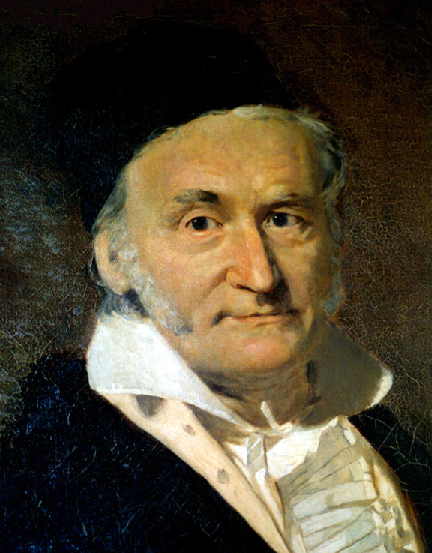
\includegraphics[width=.4\textwidth]{Gauss.pdf}
 	\end{figure}	 	
	\begin{quotation}\textrm{Carl Friedrich Gauss (1805): }
 		"The problem of distinguishing prime numbers from composite numbers and of {\color{red}resolving the latter into their prime factors} is known to be one of the most important and useful in arithmetic."
 	\end{quotation}
	 %\end{minipage}
	 %\begin{minipage}{0.3\textwidth}
	 	 %\end{minipage}
 \end{frame}
 %--- Next Frame ---%
 
 \begin{frame}{Phương pháp $p-1$ của Pollard}
 	\begin{itemize}
 		\item<+-> Phương pháp $p-1$ của Pollard cho phép ta phân tích thừa số nguyên tố của $$N=pq$$ khi 
		\[
			\color{blue} \text{tìm được  số $L$ sao cho } \quad  (p-1) \mid L  \quad \text{ và }\quad  (q-1) \nmid L.
		\]
\vspace{-0.5cm}
		\item<+-> Có nghĩa rằng, có các  số $i,j$, và $k$ với $k \not= 0$ thỏa mãn 
		\[
			\color{blue} L = i (p-1)\quad  \text{ và }\quad  L = j(q - 1) + k.
		\]  		 
 	\end{itemize}
 \end{frame}
 %--- Next Frame ---%
 
 \begin{frame}{Phương pháp $p-1$ của Pollard (2)}
 	\begin{itemize}
 		\item<+-> Theo định lý Fermat 
		\begin{align*}
			a^L &= a^{i (p-1)} = ( a^{(p-1)})^i \equiv 1^i \equiv 1 \pmod{p}, \\
			a^L &= a^{j (q-1) + k} = a^k(a^{(q-1)})^j \equiv a^k1^j \equiv a^k \pmod{q},
		\end{align*}
		và  vì $k \not= 0$, nên gần như chắc chắn  $a^k \not\equiv 1 \pmod{q}$. 
		
		\item<+-> Nói cách khác 
		\[
			p \mid (a^L -1)\qquad \text{và}\qquad q \nmid (a^L -1). 
		\] 
		\item<+-> Khi đó 
		\[
			p = \gcd (a^L -1, N).
		\] 
 	\end{itemize}
 \end{frame}
 %--- Next Frame ---%
 
 \begin{frame}
 	\begin{prblm}
 		Tìm $L$ thỏa mãn 
		\[
			(p - 1) \mid L \qquad \text{và}\qquad (q-1) \nmid L
		\]
		khi chỉ biết $N$.
 	\end{prblm}\pause 
	\begin{block}{Ý tưởng của Pollard}
			  Nếu $p -1$ là tích của nhiều  số nguyên tố nhỏ, vậy thì nó sẽ là ước của $n!$ với một số $n$ không quá lớn.
	\end{block}
 \end{frame}
 %--- Next Frame ---%
 
 \begin{frame}{Ý tưởng thuật toán Pollard}
 	\begin{itemize}
 		\item Chọn một giá trị  $n$ và  một giá trị $a$ và tính 
		\[
			d = \gcd (a^{n!} - 1, N).
		\]
		\item  Nếu $d = 1$ vậy ta thử với giá trị tiếp theo của $n$.
		\item  Nếu $d = N$ vậy ta phải thử với giá trị $a$ khác.
		\item  Nếu $1 < d < N$ vậy thì $d$ là một thừa số nguyên tố của $N$.   
 	\end{itemize}
 \end{frame}
 %--- Next Frame ---%
 
 \begin{frame}{Làm thế nào để tính $\gcd(a^{n!}-1, N)$?}
 	\begin{itemize}
 		\item<+-> Ta chỉ cần tính $a^{n!} \pmod{N}$.
 		\item<+-> Dùng đẳng thức  
		\[
			a^{(n+1)!} \equiv (a^{n!})^{n+1} \pmod{N}.
		\]
 	\end{itemize}
 \end{frame}
 
 \begin{frame}
 	\begin{block}{Thuật toán $p-1$ của Pollard}
	\qquad \textbf{Input:} Số $N$ cần phân tích thừa số nguyên tố \\
	\qquad \textbf{Output:} Một thừa số nguyên tố của $N$ 
	\begin{enumerate}[\bf 1. ]
		\item $a = 2$;\qquad\qquad\qquad    // {\color{green!70}Hoặc có thể chọn giá trị phù hợp khác} 
		
		\item \textbf{for } $j = 2,\ 3,\ 4,\ \dots,\  B$ :\qquad  // {\color{green!70}$B$ là cận xác định trước} 
		\item\qquad $a = a^j \pmod N$;
		\item\qquad $d = \gcd(a-1,N)$;
		\item \qquad \textbf{if } ($1< d< N$) \textbf{return} $d$;     
	\end{enumerate} 		
 	\end{block}
 \end{frame}
 %--- Next Frame ---%
 
 \begin{frame}
 	\begin{xmpl} 
 		\action<+->{Ta dùng thuật toán Pollard để phân tích $N = 13927189$ bắt đầu từ $\gcd(2^{9!} - 1, N)$.}
		\begin{align*}
		\action<+->{2^{9!} − 1 &\equiv 13867883 \pmod{13927189}, & \gcd(2^{9!} − 1, 13927189) &=1, \\}	
			\action<+->{2^{10!} − 1 &\equiv 5129508 \pmod{13927189}, & \gcd(2^{10!} − 1, 13927189) &=1, \\}
			\action<+->{2^{11!} − 1 &\equiv 4405233 \pmod{13927189}, & \gcd(2^{11!} − 1, 13927189) &=1, \\}	
			\action<+->{2^{12!} − 1 &\equiv 6680550 \pmod{13927189}, & \gcd(2^{12!} − 1, 13927189) &=1, \\}					
			\action<+->{2^{13!} − 1 &\equiv 6161077 \pmod{13927189}, & \gcd(2^{13!} − 1, 13927189) &=1, \\}	
			\action<+->{2^{14!} − 1 &\equiv 879290 \pmod{13927189},  & \gcd(2^{14!} − 1, 13927189) &=3823}					
		\end{align*}
		\action<+->{Vậy $p = 3823$ là một thừa số nguyên tố của $N$, còn $q = N/3823=3643$. 
		\begin{align*}
p - 1 = 3822 &= 2 \cdot 3 \cdot 7^2 \cdot 13 			\\
q - 1 = 3642 &= 2 \cdot 3 \cdot 607.} 
		\end{align*}
 	\end{xmpl}
 \end{frame}
 %--- Next Frame ---%
 
 \begin{frame}
	 \begin{xmpl}
	 	Ta dùng phương pháp của Pollard để phân tích số $N = 168441398857$.
		\begin{align*}
		\action<+->{2^{50!} − 1 &\equiv 114787431143 \pmod{N}, & \gcd(2^{50!} − 1, N) &=1, \\}	
		\action<+->{2^{51!} − 1 &\equiv 36475745067 \pmod{N}, & \gcd(2^{51!} − 1, N) &=1, \\}	
		\action<+->{2^{52!} − 1 &\equiv 67210629098 \pmod{N}, & \gcd(2^{52!} − 1, N) &=1, \\}	
		\action<+->{2^{53!} − 1 &\equiv 8182353513 \pmod{N}, & \gcd(2^{53!} − 1, N) &=350437.}
		\end{align*}
		\action<+->{Vậy dùng $2^{53!}-1$ cho ta một thừa số nguyên tố $p = 350437$, và thừa số còn lại $q = 480661$. Trong trường hợp này, $p - 1$ là tích của các thừa số nhỏ
 		\[
			p - 1 = 350436 = 2^2 \cdot 3\cdot 19\cdot 29\cdot 53.
		\]}
	 \end{xmpl}
 	
 \end{frame}
 %--- Next Frame ---%
 
 \begin{frame}{Sinh khóa cho RSA chống lại tấn công  Pollard}
Để tránh bị tấn công bằng thuật toán $p-1$ của Pollard, Bob nên sinh khóa bí mật $p$ và $q$ thỏa mãn 
\begin{quotation}
	Cả hai số $p-1$ và $q-1$ đều phải có ít nhất một thừa số nguyên tố lớn. 
\end{quotation}
Các số nguyên tố thỏa mãn tính chất này thường được gọi là các  \emph{số nguyên tố mạnh}.
 \end{frame}
 %--- Next Frame ---%
\end{document}



%%% Local Variables:
%%% mode: latex
%%% TeX-master: t
%%% End:
